%
%  exercise-1.tex
%  artificial intelligence
%
%  Created by Illya Starikov on 01/17/18.
%  Copyright 2018. Illya Starikov. All rights reserved.
%

\RequirePackage[l2tabu, orthodox]{nag}
\documentclass[12pt]{scrartcl}

\newcommand{\exercisenumber}{5}
\newcommand{\duedate}{July 24\textsuperscript{th}, 2018}
\usepackage{amssymb,amsmath,verbatim,graphicx,microtype,upquote,units,booktabs,akkwidepage}

\newcommand{\chapterNumber}[1]{
    \setcounter{section}{#1}
    \addtocounter{section}{-1}
}
\usepackage[shortlabels]{enumerate}
\usepackage{multicol}

\definecolor{dkgreen}{rgb}{0,0.6,0}
\definecolor{gray}{rgb}{0.5,0.5,0.5}
\definecolor{mauve}{rgb}{0.58,0,0.82}

\lstset{ %
  language=R,                     % the language of the code
  basicstyle=\ttfamily\footnotesize,       % the size of the fonts that are used for the code
  numbers=left,                   % where to put the line-numbers
  numberstyle=\tiny\color{gray},  % the style that is used for the line-numbers
  stepnumber=1,                   % the step between two line-numbers. If it's 1, each line
                                  % will be numbered
  numbersep=5pt,                  % how far the line-numbers are from the code
  backgroundcolor=\color{white},  % choose the background color. You must add \usepackage{color}
  showspaces=false,               % show spaces adding particular underscores
  showstringspaces=false,         % underline spaces within strings
  showtabs=false,                 % show tabs within strings adding particular underscores
  frame=single,                   % adds a frame around the code
  rulecolor=\color{black},        % if not set, the frame-color may be changed on line-breaks within not-black text (e.g. commens (green here))
  tabsize=2,                      % sets default tabsize to 2 spaces
  breaklines=true,                % sets automatic line breaking
  breakatwhitespace=false,        % sets if automatic breaks should only happen at whitespace
  keywordstyle=\color{blue},      % keyword style
  commentstyle=\color{dkgreen},   % comment style
  stringstyle=\color{mauve}      % string literal style
}

\begin{document}
\maketitle

\section{DBSCAN}
\begin{enumerate}[a)]
    \item The table would look as follows:

        \begin{table}[H]
            \centering
            \begin{tabular}{|l|c|c|c|l|}
                \hline
                \textbf{Point} & \textbf{x} & \textbf{y} & \textbf{Density} & \textbf{Designation} \\\hline
                A1 & 1 & 4 & 3 & Core Point \\
                A2 & 5 & 2 & 3 & Core Point \\
                A3 & 4 & 3 & 3 & Core Point \\
                A4 & 5 & 6 & 2 & Border Point \\
                A5 & 2 & 5 & 2 & Border Point \\
                A6 & 5 & 4 & 4 & Core Point \\
                A7 & 1 & 2 & 2 & Border Point \\
                A8 & 3 & 1 & 1 & Noise \\\hline
            \end{tabular}
        \end{table}

    \item The points in the two clusters would be:

        \begin{itemize}
            \item $\{ A1, A5, A7 \}$
            \item $\{ A2, A3, A4, A6 \}$
        \end{itemize}

        The clusters are formed by first identifying the main points; this is done via calculating the $\epsilon$, or the density of the points (i.e., how many points are around those points). After the core points have been identified, the border points are found via observing which points are close (within an $\epsilon$ value) to the core points. Finally, the remaining points are simply noise.
\end{enumerate}

\section{Bagging Vs Boosting}
\subsection{Iris}
Looking at the confusion matrix of using bagging:

\begin{verbatim}
  a  b  c   <-- classified as
 50  0  0 |  a = Iris-setosa
  0  0 50 |  b = Iris-versicolor
  0  0 50 |  c = Iris-virginica
\end{verbatim}

And comparing to the confusion matrix of boosting:

\begin{verbatim}
  a  b  c   <-- classified as
 50  0  0 |  a = Iris-setosa
  0 45  5 |  b = Iris-versicolor
  0  1 49 |  c = Iris-virginica
\end{verbatim}

We see that boosting is far more accurate; the kappa statistic agrees, where bagging had a kappa statistic of 0.5 versus the boosting kappa statistic of 0.94.

\subsection{Iris}
Looking at the confusion matrix of bagging:

\begin{verbatim}
 445  13 |   a = benign
   7 234 |   b = malignant
\end{verbatim}

And comparing to the confusion matrix of the boosting:

\begin{verbatim}
   a   b   <-- classified as
 445  13 |   a = benign
  17 224 |   b = malignant
\end{verbatim}

We see there is very little difference in accuracy. The kappa statistic agrees; where bagging had a kappa statistic of 0.937 versus the boosting kappa statistic of 0.9046.

\section{KMeans In R}
\lstinputlisting{src/problem-3.r}

\begin{figure}[H]
    \centering
    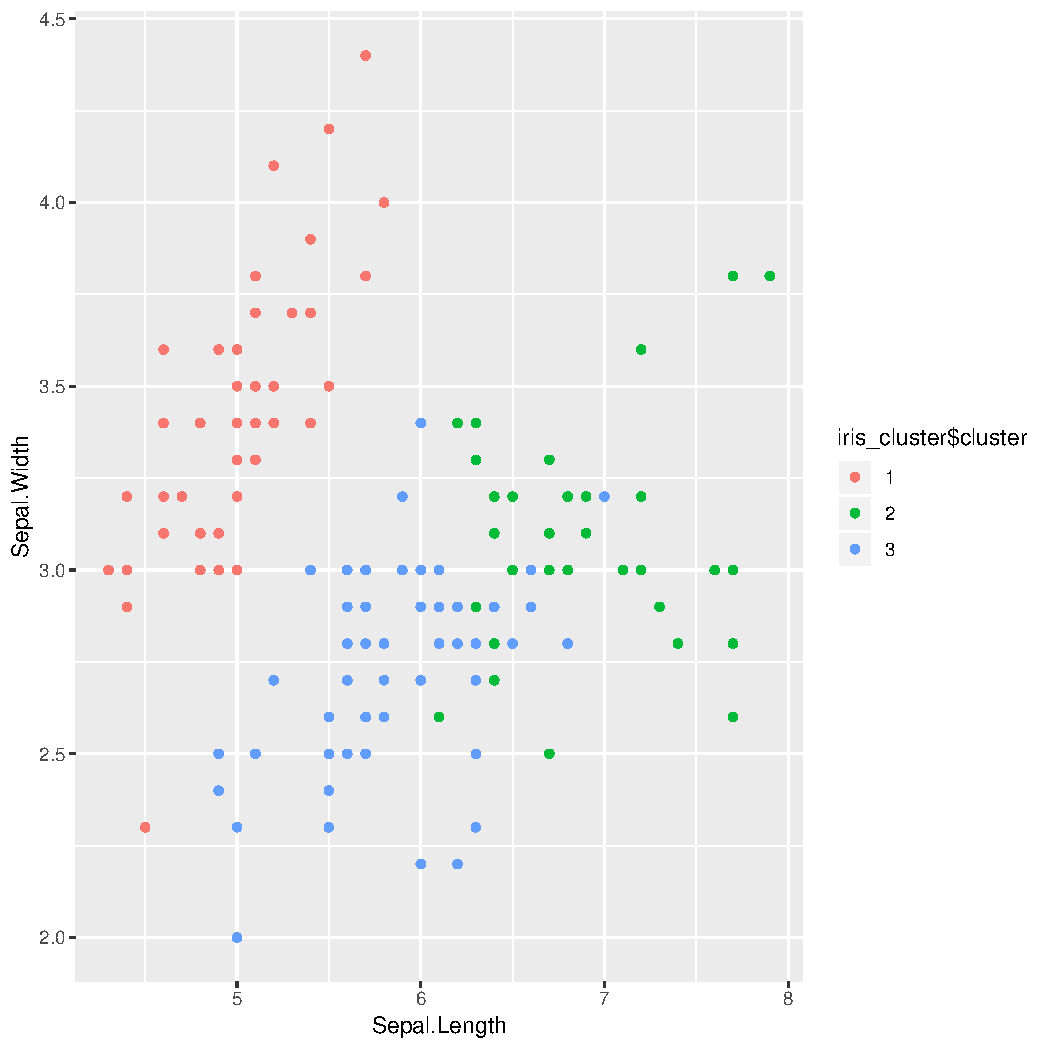
\includegraphics[width=0.8\linewidth]{assets/problem-3.pdf}
\end{figure}


\section{DBSCAN In R}
\lstinputlisting[firstline=13]{src/problem-4.r}

\begin{figure}[H]
    \centering
    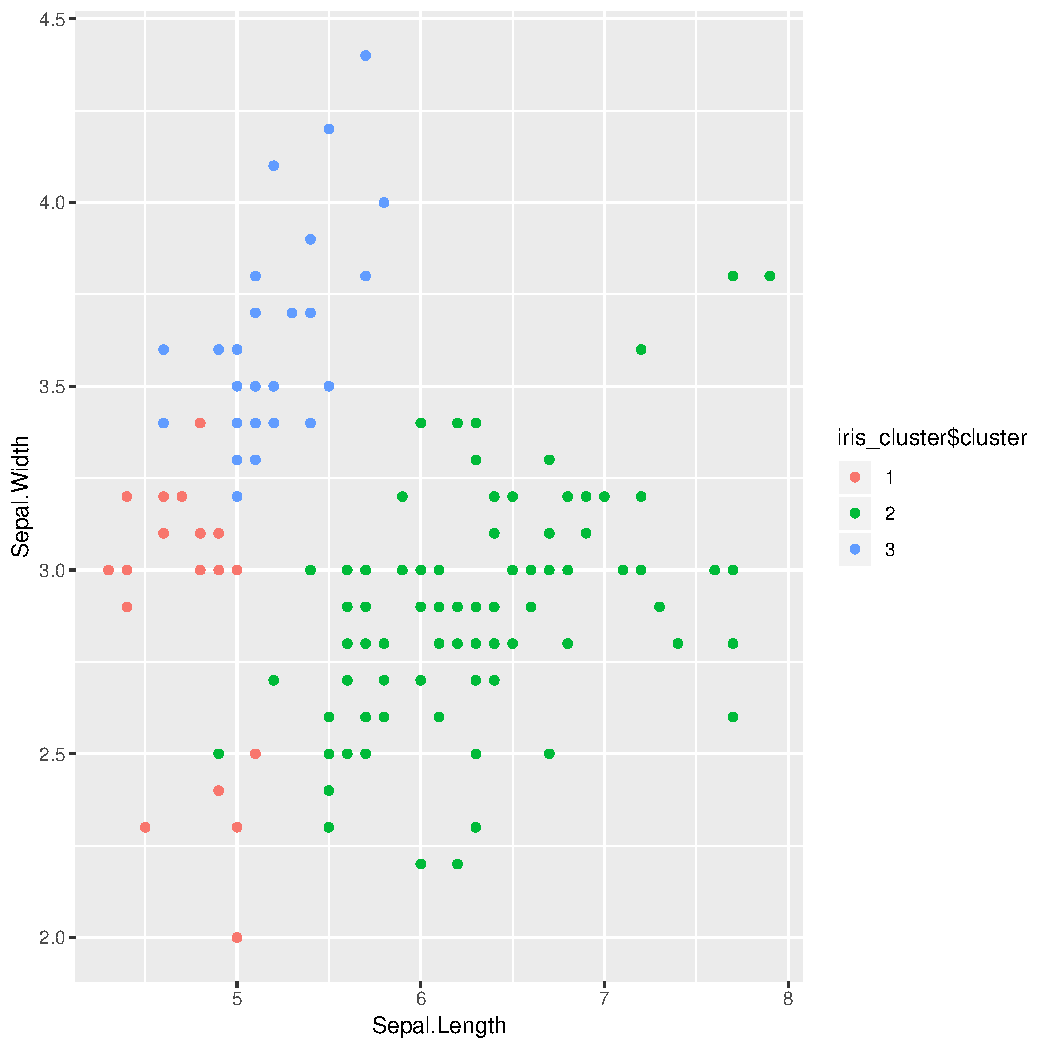
\includegraphics[width=0.8\linewidth]{assets/problem-4.pdf}
\end{figure}

\section{Frames For Days}
\lstinputlisting{src/problem-5.r}

\section{She's So Mean}
\lstinputlisting[firstline=52]{src/problem-6.r}

\section{Animals}
\lstinputlisting{src/problem-7.r}

\end{document}
